\documentclass[11pt]{article}
\usepackage{amsmath, amssymb}
\usepackage{geometry}
\geometry{margin=1in}
\usepackage{fancyhdr}
\usepackage{lastpage}
\usepackage{parskip} % Better paragraph spacing
\usepackage{titlesec} % Better section formatting
\usepackage{graphicx}
\usepackage{float}
\usepackage[most]{tcolorbox}
\usepackage{lmodern}
\usepackage{caption}

% Define commands for reusable content
\newcommand{\coursename}{CS-401 Applied Data Analysis}
\newcommand{\lecturenum}{05}
\newcommand{\lecturedate}{\today}
\newcommand{\professor}{Maria Brbic}

% Configure section spacing
\titlespacing*{\section}{0pt}{2ex plus 1ex minus .2ex}{1.5ex plus .2ex}
% Header / Footer
\pagestyle{fancy}
\fancyhf{}
\fancyhead[L]{\coursename}
\fancyhead[R]{Lecture \lecturenum}
\fancyfoot[L]{EPFL - Computer Science}
\fancyfoot[C]{Author: Jonathan Dutoit}
\fancyfoot[R]{Page \thepage\ of \pageref{LastPage}}

\begin{document}

\begin{center}
  {\large EPFL - Computer Science} \\[0.5em]
  {\Large \textbf{\coursename}} \\[0.5em]
  {\large Lecture \lecturenum\ --- \lecturedate} \\[0.5em]
  {\large Author: Jonathan Dutoit} \\[0.5em]
  {\large Professor: \professor} \\[0.5em]
\end{center}

\vspace{2cm}

\begin{center}
  {\LARGE \textbf{Regression for disentangling data}}
\end{center}

\vspace{1cm}

\section*{Linear Regression}
\begin{itemize}
	\item \textcolor{red}{Given}: n data points (X, y). where $X_i$ is k-dimensional vector of predictors (a.k.a. Features) of i-th data point, and  $y_i$ is scalar outcome
	\item \textcolor{red}{Goal}: find the optimal coefficient vector $\beta = (\beta_1, ..., \beta_k)$ for approximating the $y_i$'s as linear function of the  $X_i$'s
	\begin{center}
		\[
		y_i = X_i \beta + \epsilon_i \\
		    = \beta_I X_{i1} + ... + \beta_k X_{ik} + \epsilon_i
		.\]
		, for i = 1, ..., n
	\end{center}
	where $\epsilon_i$ are the error terms that should be as small as possible
	\item $X_n$ usually the constant 1 (by def)  $\Rightarrow$  $\beta_1$ a constant intercept
\end{itemize}
% Quick centered image
\begin{figure}[H]
    \centering
    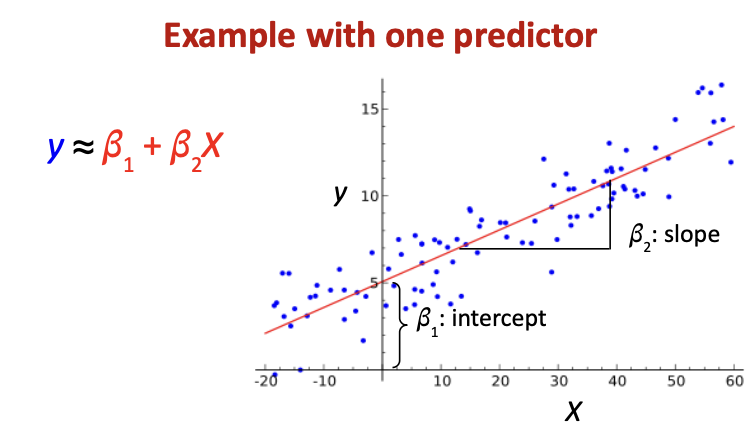
\includegraphics[width=0.8\textwidth]{linear-example}
    \label{fig:LABEL}
\end{figure}

\section*{Optimality criterion: least squares}
\begin{center}
	$y_i = X_i \beta + \epsilon_i$, for i = 1, ..., n
\end{center}
\begin{itemize}
	\item Intuitively, want errors $\epsilon_i$ to be as small as possible
	\item Technically, want sum of squared errors as small as possible $\Leftrightarrow$ find  $\hat{\beta}$ such that we minimize
\end{itemize}

\[
	\sum^{n}_{i=1}{(y_i - X_i \hat{\beta})^{2}}
.\] 

\section*{Use cases of \textcolor{red}{regression}}
\begin{itemize}
	\item \textcolor{red}{Prediction}: use fitted model to estimate outcome y for a new X not seen during model fitting 
	\item \textcolor{purple}{Descriptive data analysis}: compare average outcomes across subgroups of data (\textcolor{purple}{today!})
	\item \textcolor{blue}{Casual modeling}: understand how outcome \textit{y} changes when you manipulate predictors X \textcolor{blue}{(next lecture is about causality, although not primarily using regression)}
\end{itemize}

\vspace{1cm}
\begin{center}
  {\LARGE \textbf{Regression as comparison of average outcomes}}
\end{center}

\vspace{0.5cm}
\section*{Example with one binary predictor $X_i$}
\begin{itemize}
	\item $X_i$ = \verb|mom_hs| = "Did mother finish high school?"  $\in {0, 1}$ where 0 = No, and 1 = Yes
	\item $y_i$ = \verb|kid_score| = child's score on cognitive test  $\in [0, 140]$
\end{itemize}

\[
y_i = \textcolor{red}{\beta_i} + \textcolor{orange}{\beta_2}X_i + \epsilon_i
.\] 

\begin{center}
	\verb|kid_score| = \textcolor{red}{78} + \textcolor{orange}{12} $\cdot$ \verb|mom_hs| + error
\end{center}

% Quick centered image
\begin{figure}[H]
    \centering
    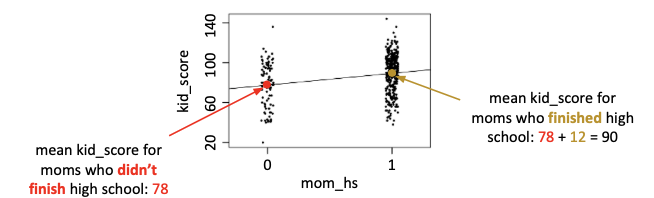
\includegraphics[width=0.7\textwidth]{example_kids}
    \label{fig:LABEL}
\end{figure}

\begin{itemize}
	\item \textcolor{red}{Intercept $\beta_1$}: mean outcome for data points i with $X_i = 0$
	\item \textcolor{orange}{Slope $\beta_2$}: difference in mean outcomes between data points with $X_i = 1$ and data points with  $X_i = 0$
	\item \textbf{Reason}: means minimize least-squares criterion: 
		\begin{center}
		$\sum^{n}_{i=1}{y_i - m}^{2}$ is minimized w.r.t. m when \\
		$-2\sum^{n}_{i=1}{(y_i - m)} = 0$, i.e., when m = $(1/n)\sum^{n}_{i=1}y_i$
		\end{center}
\end{itemize}

\begin{tcolorbox}[
  colback=yellow!15,     % background color
  colframe=black!50,    % border color
  boxrule=1pt,       % border thickness
  arc=3mm,             % rounded corners
  left=4mm, right=4mm, top=2mm, bottom=2mm % padding
]
\textbf{Mean monkey}

\vspace{0.3cm}
\textcolor{red}{So why not just compute the two means separately and them compare then?}
\end{tcolorbox}

\section*{Example with one continuous predictor $X_i$}
\begin{itemize}
	\item $X_i$ = \verb|mon_iq| = mother's IQ score  $\in [70, 140]$
	\item $y_i$ = \verb|kid_score| = child's score on cognitive test  $\in [0, 140]$ 
	\begin{center}
		$y_i = \textcolor{red}{\beta_1} + \textcolor{orange}{\beta_2}X_i + \epsilon_i$ \\
	        \verb|kid_score| = \textcolor{red}{26} + \textcolor{orange}{0.6} $\cdot$ \verb|mon_iq| + error
	\end{center}
	% Quick centered image
	\begin{figure}[H]
	    \centering
	    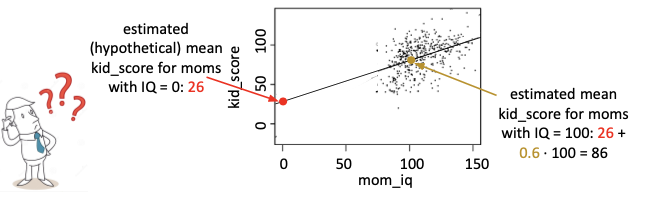
\includegraphics[width=0.8\textwidth]{continuous-predic}
	    \label{fig:LABEL}
	\end{figure}
\end{itemize}

\begin{itemize}
	\item \textcolor{red}{Intercept $\beta_1$}: estimated mean outcome for data points i with $X_i$ = 0
	\item \textcolor{orange}{Slope $\beta_2$}: difference in estimated mean outcomes between data points whose $X_i$'s differ by 1
	\item Why "estimated"? Because sometimes linear regression won't fit our data correctly...
	\item NB: for binary predictor, we got "exact"instead of "estimated"
\end{itemize}

\newpage

\section*{Example with multiple predictors}
\begin{itemize}
	\item ($X_{i1}$ = 1 = constant)
	\item $X_{i2}$ = \verb|mom_hs| = "Did mother finish high school?"  $\in {0, 1}$, where 0 = No and 1 = Yes
	\item $X_{i3}$ = \verb|kid_score| = child's score on cognitive test $\in [0. 140]$
	\item $y_i$ = \verb|kid_score| = child's score on cognitive test  $\in [0, 140]$
\end{itemize}

\begin{center}
	$y_i = \textcolor{red}{\beta_1} + \textcolor{orange}{\beta_2}X_{i2} + \textcolor{blue}{\beta_3}X_{i3} + \epsilon_i$ \\
	\verb|kid_score| = \textcolor{red}{26} + \textcolor{orange}{6} $\cdot$ \verb|mom_hs| +  \textcolor{blue}{0.6} $\cdot$ \verb|mom_iq| + error
\end{center}

% Quick centered image
\begin{figure}[H]
    \centering
    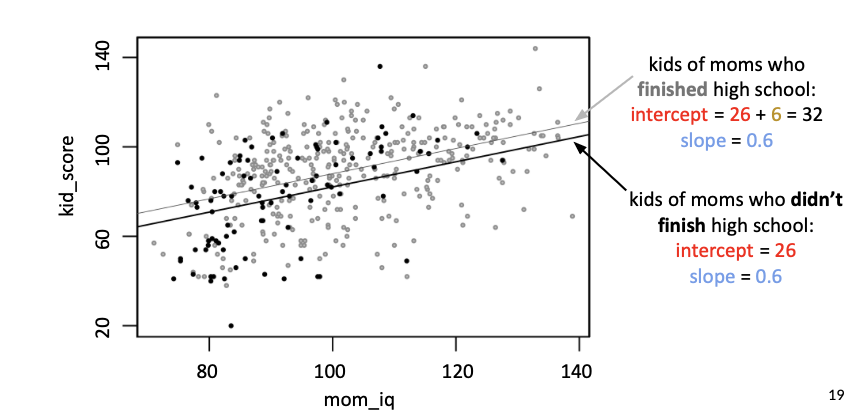
\includegraphics[width=0.8\textwidth]{multiple-predictors}
    \label{fig:LABEL}
\end{figure}

\section*{Example with \textcolor{green}{interaction} of predictors}
\begin{itemize}
	\item $X_{i2}$ = \verb|mom_hs| = "Did mother finish high school?"  $\in {0, 1}$, where 0 = No and 1 = Yes
	\item $X_{i3}$ = \verb|mom_iq| = mother's IQ score  $\in [70, 140]$
	\item $y_i$ = \verb|kid_score| = child's score on cognitive test $\in [0. 140]$
\end{itemize}

\begin{center}
	$y_i = \textcolor{red}{\beta_1} + {\textcolor{orange}{\beta_2}X_{i2} + \textcolor{blue}{\beta_3}X_{i3} + \textcolor{green}{\beta_4 X_{i2}X_{i3}} + \epsilon_i$

\texttt{kid\_score} = \textcolor{red}{-11} + \textcolor{orange}{51} $\cdot$ \texttt{mom\_hs} + \textcolor{blue}{1.1} $\cdot$ \texttt{mom\_iq} \textcolor{green}{- 0.5} $\cdot$ \textcolor{green}{\texttt{mom\_hs} $\cdot$ \texttt{mom\_iq}} + error
\end{center}

\newpage

\begin{tcolorbox}[
  colback=gray!15,     % background color
  colframe=black!50,    % border color
  boxrule=1pt,       % border thickness
  arc=3mm,             % rounded corners
  left=4mm, right=4mm, top=2mm, bottom=2mm % padding
]
\textbf{So why not just compute the two means separately and then compare them?}
\end{tcolorbox}
\begin{minipage}{0.8\textwidth}
% Quick centered image
\begin{figure}[H]
    \centering
    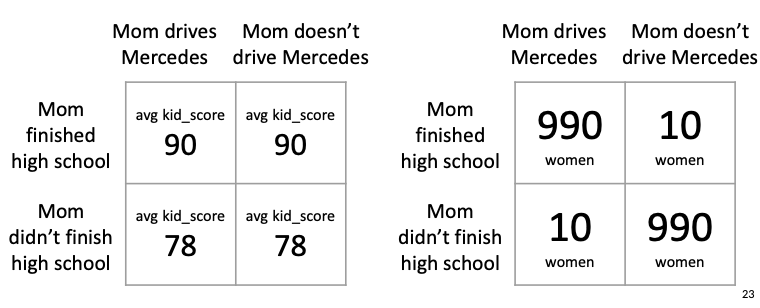
\includegraphics[width=\linewidth]{mercedes}
    \label{fig:LABEL}
\end{figure}
\end{minipage}
\hfill
\begin{minipage}{0.2\textwidth}
\centering
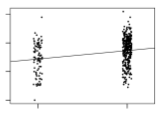
\includegraphics[width=\linewidth]{example-kids-2}
\end{minipage}
\begin{itemize}
	\item Mean \verb|kid_score| for Mercedes drives: \textbf{0.99 $\cdot$ 90 + 0.01  $\cdot$ 78  $\approx$ 90}
	\item Mean \verb|kid_score| for non-Mercedes drives: \textbf{0.01 $\cdot$ 90 + 0.99 $\cdot$ 78  $\approx$ 78}
	\item But really driving Mercedes makes no difference (for fixed high-school predictor)!
	\item Root of evil: \textbf{correlation} between finishing high school and driving Mercedes
	\item \textbf{Regression} to the rescue: \textbf{\texttt{kid\_score} = \textcolor{red}{78} + \textcolor{orange}{12} $\cdot$ \texttt{mom\_hs} +  \textcolor{green}{0} $\cdot$ mercedes + error}
\end{itemize}

\newpage
\begin{center}
  {\LARGE \textbf{Quantifying uncertainty}}
\end{center}

\begin{itemize}
	\item Statistical software gives you more than just coefficient $\textcolor{blue}{\beta}$:
\end{itemize}

% Quick centered image
\begin{figure}[H]
    \centering
    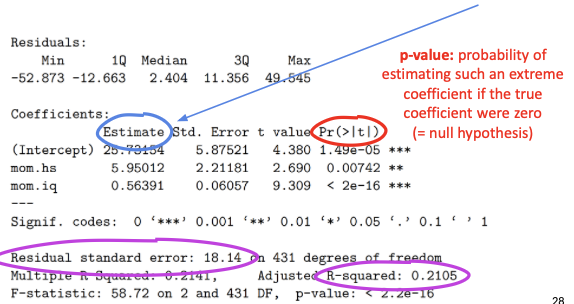
\includegraphics[width=0.5\textwidth]{statistical-software}
    \label{fig:LABEL}
\end{figure}

\section*{Residuals and $R^{2}$}
\begin{itemize}
	\item \textcolor{purple}{Residual} for data point \textit{i}: estimation error on data point \textit{i}: 
		\begin{center}
			$r_i = y_i - X_i \hat{\beta}$
		\end{center}
	\item Mean of residuals = 0 (total overestimation = total underestimation)
	\item Variance of residuals \\
	= avg squared distance of predicted value from observed value \\
	= "\textcolor{blue}{unexplained variance}"
\item Fraction of variance explained by the model: 
\end{itemize}

\begin{center}
	$R^{2} = 1 - \textcolor{blue}{\hat{\sigma^{2}}} / \textcolor{red}{s^{2}_y}$, \textcolor{red}{variance of outcomes y}
\end{center}

% Quick centered image
\begin{figure}[H]
    \centering
    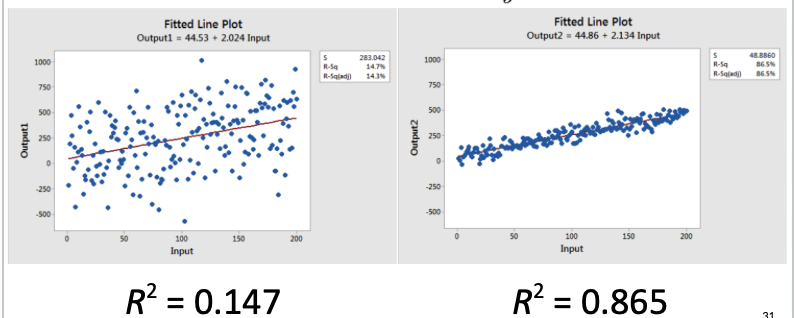
\includegraphics[width=0.8\textwidth]{r2}
    \label{fig:LABEL}
\end{figure}

% Quick centered image
\begin{figure}[H]
    \centering
    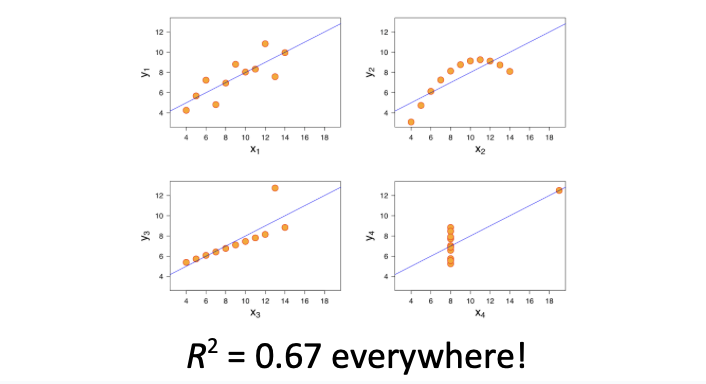
\includegraphics[width=0.7\textwidth]{r2-2}
    \label{fig:LABEL}
\end{figure}

\vspace{1cm}
\begin{center}
  {\LARGE \textbf{Assumptions made in regression modeling}}
\end{center}

\vspace{1cm}

1. Validity: 
\begin{itemize}
	\item a) Outcome measure should accurately reflect the phenomenon of interest
	\item b) Model should include all relevant predictors
	\item c) Model should generalize to cases to which it will be applied
\end{itemize}
\begin{minipage}{0.7\textwidth}
2. Linearity: \\ 
\[
	y_i = \beta_i X_{i1} + ... + \beta_k X_{ik} + \epsilon_i, \text{for i = 1, ..., n}
.\]

But very flexible: we require linearity in predictors (not necessarily in raw inputs); predictors can be arbitrary functions of raw inputs, e.g., 
\begin{itemize}
	\begin{itemize}
		\item logarithms, polynomials, reciprocals, ...
		\item interactions (i.e., products) of multiple inputs
		\item discretization of raw inputs, coded as indicator variables
	\end{itemize}
\end{itemize}
\end{minipage}
\hfill
\begin{minipage}{0.3\textwidth}
\centering
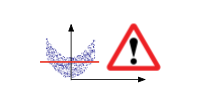
\includegraphics[width=\linewidth]{linear-except}
\end{minipage}

3. Independence of errors: no interaction between data points

4. Equal variance of errors

5. Normality (Gaussianity) of errors

\textbf{Note:} (4) and (5) are less important in practice

\newpage
\begin{center}
  {\LARGE \textbf{Transformations of predictors and outcomes}}
\end{center}

\vspace{0.5cm}

\section*{Transformations of predictors}
\begin{itemize}
	\item When we apply \textbf{linear transformations} to predictors, the model remains "equally good"
		\begin{itemize}
			\item The fitted coefficients may change, but predicted outcomes and model fit ($R^{2}$) won't change
	\end{itemize}
\end{itemize}

\section*{Mean-centering of predictors}
\begin{itemize}
	\item Compute the mean value of a predictor over all data points, and substract it from each value of that predictor: \\
		$X_{ij} \Leftarrow X_{ij} - mean(X_{1j}, ..., X_{nj})$
	\item $\Rightarrow$ the predictor  $X_{ij}$ now has mean 0
\end{itemize}
% Quick centered image
\begin{figure}[H]
    \centering
    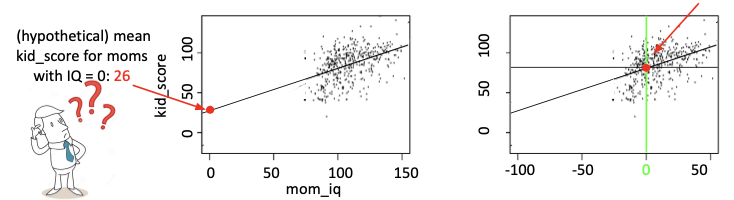
\includegraphics[width=0.8\textwidth]{mean-centering}
    \label{fig:LABEL}
\end{figure}

mean \verb|kid_score| for moms with mean IQ: \textcolor{red}{86}

\textcolor{red}{After mean-centering of predictors}, you have a convenient interpretation of coefficients $\beta_j$ of main predictors (i.e., non-interaction predictors):
 \begin{itemize}
	\item j = 1 (i.e., intercept):
		\begin{itemize}
			\item Estimated mean outcome when each predictor has its mean value
		\end{itemize}
	\item j $>$ 1 
		\begin{itemize}
			\item Model w/o interactions: estimated mean increase in outcome \textit{y} for each unit increase in $X_{ij}$
			\item Model with interactions: estimated mean increase in outcome \textit{y} for each unit increase in $X_{ij}$  \textbf{when each other predictor has its mean value}
		\end{itemize}
\end{itemize}

\section*{Standardization via z-scores}

\begin{itemize}
	\item First \textcolor{purple}{mean-center} all predictors, then \textcolor{blue}{divide them by their standard deviations}:
	\begin{center}
	$X_{ij} \Leftarrow [X_{ij} - mean(X_{1j}, ..., X_{nj})] / sd(X_{1j}, ..., X_{nj})}$
	\end{center}
	\item Resulting values are called "\textbf{z-scores}"
	\item All predictors now have the same units: \\
	distance (in terms of standard deviations) from the mean
\item This lets us compare coefficients for predictors with previously incomparable units of measurement, e.g., IQ score vs. earnings in Swiss francs vs. height in centimeters
\end{itemize}
\section*{Logarithmic outcomes}
\begin{itemize}
	\item \textcolor{green}{Pratical}: makes sense if the outcome y follows a heavy-tailed distribution (power-law)
	\item Only works for non-negative outcomes
	\item \textcolor{red}{Theoretical}: turns an additive model into a \textcolor{blue}{multiplicative model}:
	\begin{center}
		$\log{y_i} = b_0 + b_1X_{i1} + b_2X_{i2} + ... + \epsilon_i$ 
	\end{center}
	
	Exponentiating both sides yields 
	\begin{center}
	$y_i = e^{b_0 + b_1X_{i1} + b_2X_{i2} + ... + \epsilon_i}$ \\
	$= B_0 \cdot B_1^{X_{i1}} \cdot B_2^{X_{i2}} \cdot \cdot \cdot E_i$
	\end{center}
\end{itemize}

\textbf{\textcolor{red}{interpreting coefficients}}

\begin{itemize}
	\item An \textcolor{green}{additive} increase of 1 in predictor $X_i1$ is associated with a \textcolor{orange}{multiplicative} increase of $B_1 := exp(b_1)$ in the outcome
	\item If $b_1 \approx 0$, we can immediately interpret  $b_1$ (without needing to exponentiate it first to get  $B_1$!) as the  \textcolor{blue}{relative increase} in outcomes, since $exp(b_1) \approx 1 + b_1$
	\item E.g., $b_1 = 0.05 \Rightarrow$ $B_1$ = exp($b_1$)  $\approx$ 1.05 \\
		$\Rightarrow$ "+1 in predictor  $X_{-1}$"is associated with "+5\% in outcome"
\end{itemize}

\vspace{1cm}
\begin{center}
  {\LARGE \textbf{Going beyond linear regression for comparing means}}
\end{center}

\vspace{1cm}
\section*{Generalized linear models}
\begin{itemize}
	\item Logistic regression: binary outcomes
	\item Poisson regression: non-negative integer outcomes (e.g., counts)
\end{itemize}

\begin{minipage}{0.6\textwidth}
\begin{itemize}
	\item Two groups: P, S
	\item At time 2, group P receives a \textbf{treatment}, group S doesn't 
	\item Question: Did the treatment have an \textbf{effect?} If so, how large was it?
	\item P and S don't start out the same at time 1
	\item There is a temporal "baseline effect" even w/o treatment
\end{itemize}

\end{minipage}
\hfill
\begin{minipage}{0.4\textwidth}
\centering
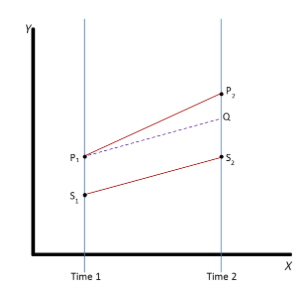
\includegraphics[width=\linewidth]{casuality-1}
\end{minipage}

\begin{minipage}{0.6\textwidth}
\begin{itemize}
	\item Elegant linear model with binary predictors:
		\begin{center}
			\textbf{$y_{it} = \textcolor{red}{a} + \textcolor{blue}{b} \cdot treated_i + \textcolor{orange}{c} \cdot time2_t + \textcolor{green}{d} \cdot (treated_i \cdot time2_t) + error_i$}
		\end{center}
	\item \textcolor{green}{d} = treatment effect
	\item All of this with one single regression!
	\item You get quantification of uncertainty (significance) for free!
\end{itemize}

\end{minipage}
\hfill
\begin{minipage}{0.4\textwidth}
\centering
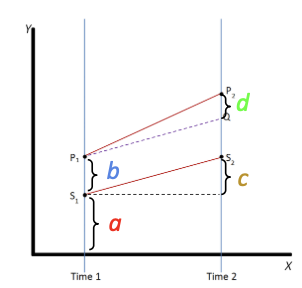
\includegraphics[width=\linewidth]{casuality-2}
\end{minipage}
\end{document}
